\documentclass{beamer}

\usepackage[T1]{fontenc}
\usepackage{inputenc}

\usepackage{tikz}
\usetikzlibrary{arrows,snakes,backgrounds,patterns,matrix,shapes,fit,calc,shadows,plotmarks}

\usepackage{amsmath}
\usepackage{listings}
\lstset{
    basicstyle=\footnotesize,
    language=Caml,
    showstringspaces=false,
}


\usetheme{Boadilla}
\usecolortheme{dolphin}
\useoutertheme{infolines}

\setbeamertemplate{footline}{
    \leavevmode%
    \hbox{%
    \begin{beamercolorbox}[wd=.333333\paperwidth,ht=2.25ex,dp=1ex,center]{author in head/foot}%
        \usebeamerfont{author in head/foot}\insertshortauthor%~~\beamer@ifempty{\insertshortinstitute}{}{(\insertshortinstitute)}
    \end{beamercolorbox}%
    \begin{beamercolorbox}[wd=.333333\paperwidth,ht=2.25ex,dp=1ex,center]{title in head/foot}%
        \usebeamerfont{title in head/foot}\insertshorttitle
    \end{beamercolorbox}%
    \begin{beamercolorbox}[wd=.333333\paperwidth,ht=2.25ex,dp=1ex,right]{date in head/foot}%
        \usebeamerfont{date in head/foot}\insertshortdate{}\hspace*{2em}
        \insertframenumber{} / \inserttotalframenumber\hspace*{2ex}
    \end{beamercolorbox}}%
    \vskip0pt%
}


\newcommand{\TODO}{{\color{red}\bf [TODO]}}
\graphicspath{ {assets/} }


\title{Intruder models and attack scenarios}
\author{Maxime Puys \and Marie-Laure Potet}
\date{\today}


\begin{document}

\begin{frame}
    \maketitle
\end{frame}

\begin{frame}
    \frametitle{Objectives}

    \begin{figure}[htb]
        \centering
        \resizebox {!} {.7\textheight} {
            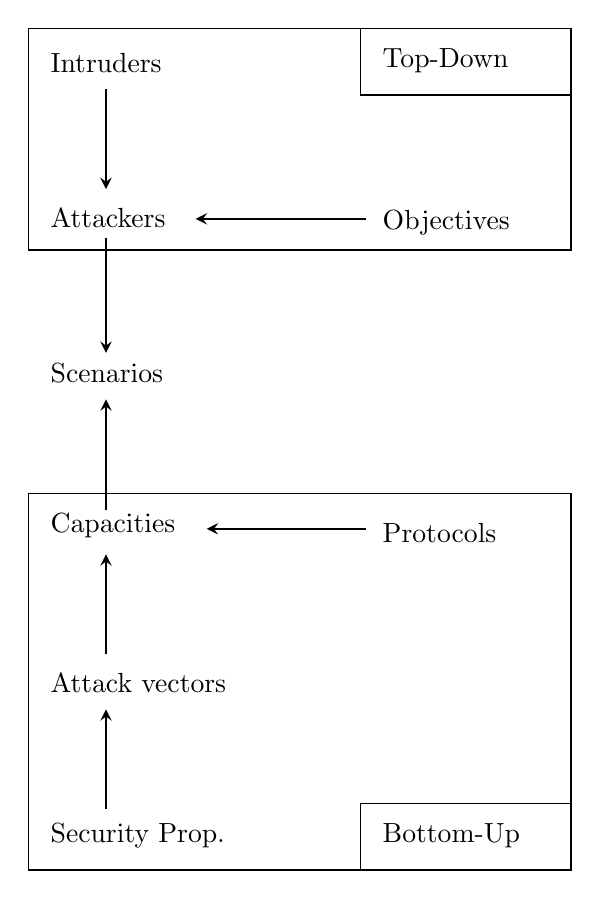
\begin{tikzpicture}[y=0.80pt, x=0.80pt, yscale=-1.000000, xscale=1.000000, inner sep=0pt, outer sep=0pt,
        arrow/.style={thick,->,shorten >=2pt,shorten <=2pt,>=stealth},
    ]
    \path[draw=black,miter limit=4.00,line width=0.600pt,rounded corners=0.0000cm] (40,40)  rectangle (285,140);
    \path[draw=black,miter limit=4.00,line width=0.600pt,rounded corners=0.0000cm] (190,40) rectangle (285,70);

    \path[fill=black] (50,60)   node[above right] (text2987) {Intruders};
    \path[fill=black] (200,60)  node[above right] (text2991) {Top-Down};
    \path[fill=black] (50,130)  node[above right] (text2995) {Attackers};
    \path[fill=black] (200,133) node[above right] (text2999) {Objectives};


    \draw[arrow] (75,65) -- (75,115) node {}; % Intruder -- Attacker
    \draw[arrow] (195,126) -- (113,126) node {}; % Objectives -- Attacker

    \draw[arrow] (75,132) -- (75,189) node {}; % Attacker -- Scenarii
    \path[fill=black] (50,200) node[above right] (text3005) {Scenarios};
    \draw[arrow] (75,260) -- (75,205) node {}; % Capacities -- Scenarii

    \path[draw=black,miter limit=4.00,line width=0.600pt,rounded corners=0.0000cm] (40,250)  rectangle (285,420);
    \path[draw=black,miter limit=4.00,line width=0.600pt,rounded corners=0.0000cm] (190,390) rectangle (285,420);

    \path[fill=black] (50,270)  node[above right] (text3023) {Capacities};
    \path[fill=black] (50,340)  node[above right] (text3009) {Attack vectors};
    \path[fill=black] (50,410)  node[above right] (text3019) {Security Prop.};
    \path[fill=black] (200,272) node[above right] (text3013) {Protocols};
    \path[fill=black] (200,410) node[above right] (text3029) {Bottom-Up};

    \draw[arrow] (75,325)  -- (75,275)  node {}; % Attack vectors -- Capacities
    \draw[arrow] (75,395)  -- (75,345)  node {}; % Security props -- Attack vectors
    \draw[arrow] (195,266) -- (118,266) node {}; % Protocols -- Capacities
\end{tikzpicture}

        }
        \caption{Chosen approach}
    \end{figure}
\end{frame}

\section{Top-down approach}

\begin{frame}
    \frametitle{Table of contents}

    \tableofcontents[currentsection]
\end{frame}

\begin{frame}
    \frametitle{Architecture}

    \begin{figure}
        \centering
        \resizebox {\columnwidth} {!} {
            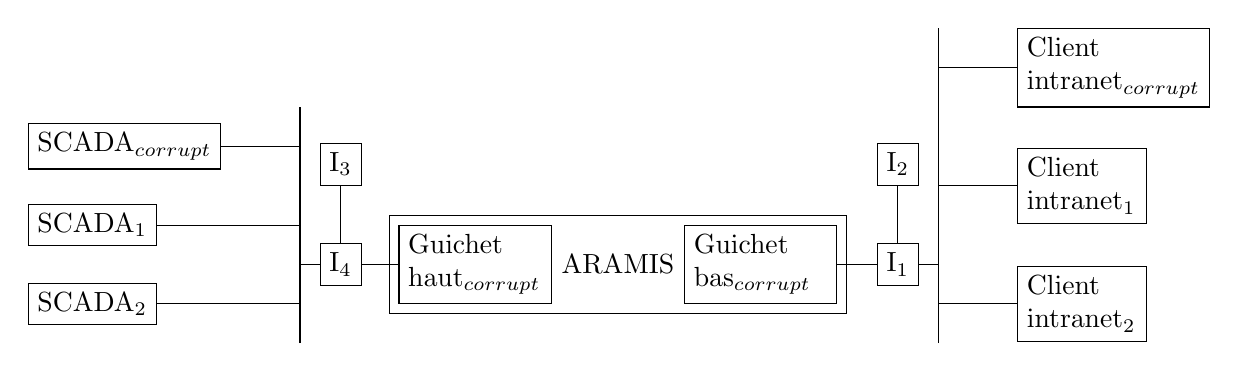
\begin{tikzpicture}[
        typetag/.style={rectangle, draw}
    ]
    %\draw [help lines] (0,0) grid (10,10);

    \node[draw, anchor=west] (SCADA2) at (0,0.5){SCADA$_{2}$}; 
    \node[draw, anchor=west] (SCADA1) at (0,1.5){SCADA$_{1}$}; 
    \node[draw, anchor=west] (SCADAc) at (0,2.5){SCADA$_{corrupt}$};
    
    \coordinate (bus0) at ($(1,0)+(SCADAc.east |- 42,0)$);
    \draw (bus0) -- (bus0 |- 42,3);

    \draw (SCADA2.east) -- (bus0 |- SCADA2.east);
    \draw (SCADA1.east) -- (bus0 |- SCADA1.east);
    \draw (SCADAc.east) -- (bus0 |- SCADAc.east);

    \node[draw, anchor=west] (I4) at ($(0.25,0)+(bus0 |- 42,1)$){I$_{4}$};

    \node[anchor=west, typetag, text width=1.7cm] (GHc) at ($(1.25,0)+(bus0 |- 42,1)$) {Guichet haut$_{corrupt}$};
    \node[anchor=west] (ARAMIS) at (GHc.east){ARAMIS};
    \node[anchor=west, typetag, text width=1.7cm] (GBc) at (ARAMIS.east) {Guichet bas$_{corrupt}$};
    \node[draw, fit={(ARAMIS) (GHc) (GBc)}] {};

    \draw (bus0 |- I4.west) -- (I4.west);
    \draw (I4.east) -- (GHc.west);

    \node[draw] (I3) at ($(I4.north)+(0,1)$){I$_{3}$};
    \draw (I3.south) -- (I4.north);
    
    \node[draw, anchor=west] (I1) at ($(0.5,0)+(GBc.east |- 42,1)$){I$_{1}$};
    
    \coordinate (bus1) at ($(0.25,0)+(I1.east |- 42,0)$);
    \draw (bus1) -- (bus1 |- 42,4);

    \draw (GBc.east) -- (I1.west);

    \node[draw] (I2) at ($(I1.north)+(0,1)$){I$_{2}$};
    \draw (I2.south) -- (I1.north);

    \node[draw, anchor=west, text width=1.4cm] (CLIENT2) at ($(1,0)+(bus1 |- 42,0.5)$){Client intranet$_{2}$};
    \node[draw, anchor=west, text width=1.4cm] (CLIENT1) at ($(1,0)+(bus1 |- 42,2)$){Client intranet$_{1}$};
    \node[draw, anchor=west, text width=2.2cm] (CLIENTc) at ($(1,0)+(bus1 |- 42,3.5)$){Client intranet$_{corrupt}$};
    
    \draw (I1.east) -- (bus1 |- I1.east);
    \draw (CLIENT2.west) -- (bus1 |- CLIENT2.west);
    \draw (CLIENT1.west) -- (bus1 |- CLIENT1.west);
    \draw (CLIENTc.west) -- (bus1 |- CLIENTc.west);
\end{tikzpicture}

        }
        \caption{Possible positions for intruder}
    \end{figure}
\end{frame}

\begin{frame}
    \frametitle{Architecture (VPN mode)}

    \begin{figure}
        \centering
        \resizebox {\columnwidth} {!} {
            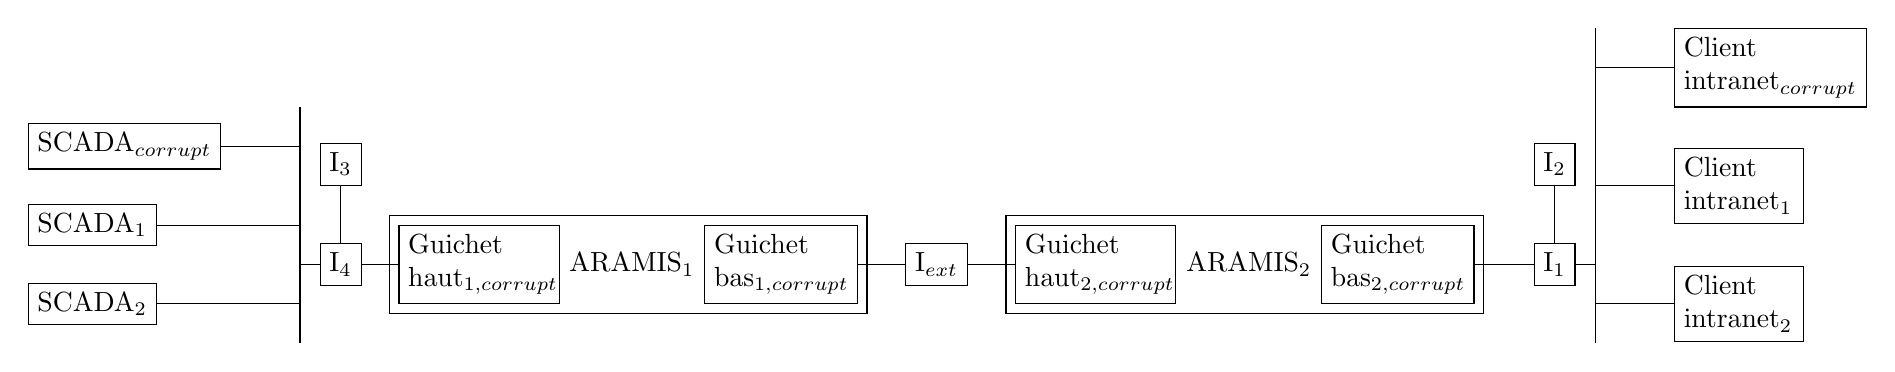
\begin{tikzpicture}[
        typetag/.style={rectangle, draw}
    ]
    %\draw [help lines] (0,0) grid (10,10);

    \node[draw, anchor=west] (SCADA2) at (0,0.5){SCADA$_{2}$}; 
    \node[draw, anchor=west] (SCADA1) at (0,1.5){SCADA$_{1}$}; 
    \node[draw, anchor=west] (SCADAc) at (0,2.5){SCADA$_{corrupt}$};
    
    \coordinate (bus0) at ($(1,0)+(SCADAc.east |- 42,0)$);
    \draw (bus0) -- (bus0 |- 42,3);

    \draw (SCADA2.east) -- (bus0 |- SCADA2.east);
    \draw (SCADA1.east) -- (bus0 |- SCADA1.east);
    \draw (SCADAc.east) -- (bus0 |- SCADAc.east);
    
    \node[draw, anchor=west] (I4) at ($(0.25,0)+(bus0 |- 42,1)$){I$_{4}$};

    \node[anchor=west, typetag, text width=1.8cm] (GH1c) at ($(1.25,0)+(bus0 |- 42,1)$) {Guichet haut$_{1,corrupt}$};
    \node[anchor=west] (ARAMIS1) at (GH1c.east){ARAMIS$_{1}$};
    \node[anchor=west, typetag, text width=1.7cm] (GB1c) at (ARAMIS1.east) {Guichet bas$_{1,corrupt}$};
    \node[draw, fit={(ARAMIS1) (GH1c) (GB1c)}] {};

    \draw (bus0 |- I4.west) -- (I4.west);
    \draw (I4.east) -- (GH1c.west);

    \node[draw] (I3) at ($(I4.north)+(0,1)$){I$_{3}$};
    \draw (I3.south) -- (I4.north);

    \node[draw] (Iext) at ($(GB1c.east)+(1,0)$){I$_{ext}$};
    \draw (Iext.west) -- (GB1c);

    \node[anchor=west, typetag, text width=1.8cm] (GH2c) at ($(1,0)+(Iext |- 42,1)$) {Guichet haut$_{2,corrupt}$};
    \node[anchor=west] (ARAMIS2) at (GH2c.east){ARAMIS$_{2}$};
    \node[anchor=west, typetag, text width=1.7cm] (GB2c) at (ARAMIS2.east) {Guichet bas$_{2,corrupt}$};
    \node[draw, fit={(ARAMIS2) (GH2c) (GB2c)}] {};

    \draw (Iext.east |- GH2c.west) -- (GH2c.west);
    
    \node[draw, anchor=west] (I1) at ($(0.751,0)+(GB2c.east |- 42,1)$){I$_{1}$};
    
    \coordinate (bus2) at ($(0.25,0)+(I1.east |- 42,0)$);
    \draw (bus2) -- (bus2 |- 42,4);

    \draw (GB2c.east) -- (I1.west);

    \node[draw] (I2) at ($(I1.north)+(0,1)$){I$_{2}$};
    \draw (I2.south) -- (I1.north);

    \node[draw, anchor=west, text width=1.4cm] (CLIENT2) at ($(1,0)+(bus2 |- 42,0.5)$){Client intranet$_{2}$};
    \node[draw, anchor=west, text width=1.4cm] (CLIENT1) at ($(1,0)+(bus2 |- 42,2)$){Client intranet$_{1}$};
    \node[draw, anchor=west, text width=2.2cm] (CLIENTc) at ($(1,0)+(bus2 |- 42,3.5)$){Client intranet$_{corrupt}$};
    
    \draw (I1.east) -- (bus2 |- I1.east);
    \draw (CLIENT2.west) -- (bus2 |- CLIENT2.west);
    \draw (CLIENT1.west) -- (bus2 |- CLIENT1.west);
    \draw (CLIENTc.west) -- (bus2 |- CLIENTc.west);
\end{tikzpicture}

        }
        \caption{Possible positions for intruder (VPN mode)}
    \end{figure}
    \vfill
    \begin{block}{More formally}
        $\mathcal{I}$ = Set of possible intruders.
    \end{block}
\end{frame}

\begin{frame}
    \frametitle{Intruder objectives 1/2}

    All intruders start with the same objectives:
    \begin{itemize}
        \item (Disp) Disponibility of ARAMIS.
        \item (Disp) Disponibility of process devices.
        \item (Disp) Disponibility of SCADA.
        \item (Int) Send modified requests to process devices.
        \item (Int) Send modified responses to SCADA.
        \item (Int) Modify configuration of ARAMIS.
        \item (Int) Modify configuration of process devices.
        \item (Int) Modify configuration of SCADA.
        \item (Auth) Send forged requests to process devices.
        \item (Auth) Send forged responses to SCADA.
    \end{itemize}
\end{frame}

\begin{frame}
    \frametitle{Intruder objectives 2/2}

    All intruders start with the same objectives:
    \begin{itemize}
        \item (Conf) Spy on requests.
        \item (Conf) Spy on responses.
        \item (Int) Replay previous requests.
        \item (Int) Replay previous responses.
    \end{itemize}
    \vfill
    \begin{block}{More formally}
        $\mathcal{O}$ = Set of possible objectives.
    \end{block}
\end{frame}

\begin{frame}
    \frametitle{Attackers 1/2}
    
    \begin{block}{Attacker}
        An {\em attacker} is an {\em intruder} with an {\em objective}.
    \end{block}
    \vfill
    \begin{block}{More formally}
        $$\mathcal{A} = \{a_{io} = (i,o) | \mathcal{R}_{1}(i,o) = 1, \forall i \in \mathcal{I}, \forall o \in \mathcal{O}\}$$
        Where $\mathcal{R}_{1}$ is the binary relation between an intruder $i$ and an objective $o$ and
        $\mathcal{R}_{1}(i,o) = 1$ if $i$ seeking for $o$ is considered, $0$ else.
    \end{block}
\end{frame}

\begin{frame}
    \frametitle{Attackers 2/2}

    Depending on their position:
    \begin{itemize}
        \item Some attack objectives are impossible to fulfill.
        \begin{itemize}
            \item An attacker cannot replay message if he did not see them earlier.
        \end{itemize}
        \item Some attack objectives are impossible to avoid.
        \begin{itemize}
            \item An attacker on the same side of the module than its target.
        \end{itemize}
    \end{itemize}
    \vfill
    \begin{block}{Conclusion}
        Thus we obtain the set of {\em attackers} $\mathcal{A}$ to consider.
    \end{block}
\end{frame}

\begin{frame}
    \frametitle{Objectives}

    \begin{figure}[htb]
        \centering
        \resizebox {!} {.7\textheight} {
            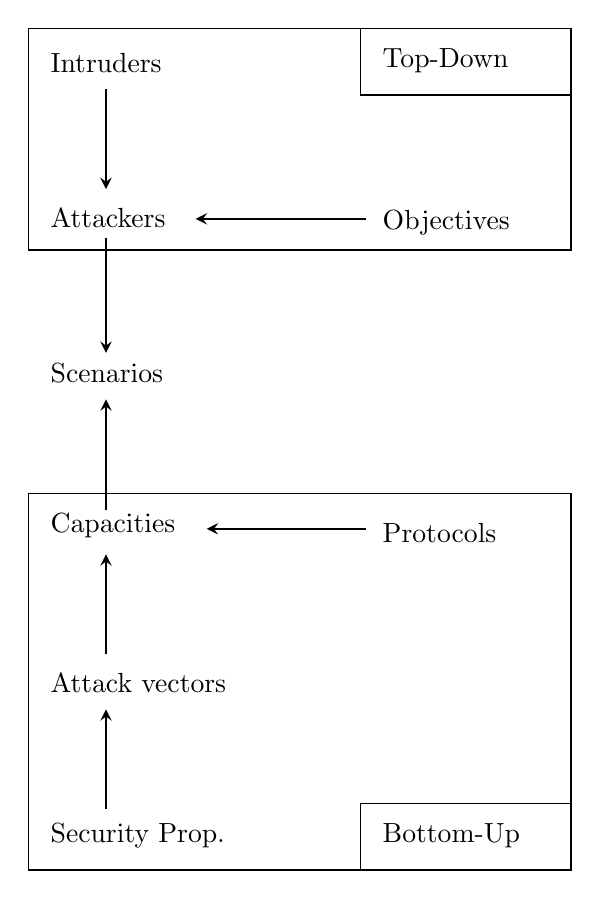
\begin{tikzpicture}[y=0.80pt, x=0.80pt, yscale=-1.000000, xscale=1.000000, inner sep=0pt, outer sep=0pt,
        arrow/.style={thick,->,shorten >=2pt,shorten <=2pt,>=stealth},
    ]
    \path[draw=black,miter limit=4.00,line width=0.600pt,rounded corners=0.0000cm] (40,40)  rectangle (285,140);
    \path[draw=black,miter limit=4.00,line width=0.600pt,rounded corners=0.0000cm] (190,40) rectangle (285,70);

    \path[fill=black] (50,60)   node[above right] (text2987) {Intruders};
    \path[fill=black] (200,60)  node[above right] (text2991) {Top-Down};
    \path[fill=black] (50,130)  node[above right] (text2995) {Attackers};
    \path[fill=black] (200,133) node[above right] (text2999) {Objectives};


    \draw[arrow] (75,65) -- (75,115) node {}; % Intruder -- Attacker
    \draw[arrow] (195,126) -- (113,126) node {}; % Objectives -- Attacker

    \draw[arrow] (75,132) -- (75,189) node {}; % Attacker -- Scenarii
    \path[fill=black] (50,200) node[above right] (text3005) {Scenarios};
    \draw[arrow] (75,260) -- (75,205) node {}; % Capacities -- Scenarii

    \path[draw=black,miter limit=4.00,line width=0.600pt,rounded corners=0.0000cm] (40,250)  rectangle (285,420);
    \path[draw=black,miter limit=4.00,line width=0.600pt,rounded corners=0.0000cm] (190,390) rectangle (285,420);

    \path[fill=black] (50,270)  node[above right] (text3023) {Capacities};
    \path[fill=black] (50,340)  node[above right] (text3009) {Attack vectors};
    \path[fill=black] (50,410)  node[above right] (text3019) {Security Prop.};
    \path[fill=black] (200,272) node[above right] (text3013) {Protocols};
    \path[fill=black] (200,410) node[above right] (text3029) {Bottom-Up};

    \draw[arrow] (75,325)  -- (75,275)  node {}; % Attack vectors -- Capacities
    \draw[arrow] (75,395)  -- (75,345)  node {}; % Security props -- Attack vectors
    \draw[arrow] (195,266) -- (118,266) node {}; % Protocols -- Capacities
\end{tikzpicture}

        }
        \caption{Chosen approach}
    \end{figure}
\end{frame}

\section{Bottom-Up approach}

\begin{frame}
    \frametitle{Table of contents}

    \tableofcontents[currentsection]
\end{frame}

\begin{frame}
    \frametitle{Security properties}

    The security properties considered are:
    \vfill
    \begin{itemize}
        \item Confidentiality
        \begin{itemize}
            \item An attacker cannot read a message.
        \end{itemize}
        \vfill
        \item Authentication
        \begin{itemize}
            \item An attacker cannot impersonate another agent of the network.
        \end{itemize}
        \vfill
        \item Integrity
        \begin{itemize}
            \item An attacker cannot modify the content of a message.
        \end{itemize}
        \vfill
        \item Fraichness
        \begin{itemize}
            \item An attacker cannot replay a message already sent.
        \end{itemize}
    \end{itemize}
    \vfill
    \begin{block}{Availability}
        {\em Availability} can be attacked through sending one or more message.\\
        Thus it can be subsummed by {\em authentication} or {\em fraichness}.
    \end{block}
\end{frame}

\begin{frame}
    \frametitle{Industrial protocols}

    Let $\mathcal{P}$ be the list of all protocols considered within the system (example):
    \begin{itemize}
        \item Modbus-TCP
        \item OPC-UA
        \item FTP
        \item HTTPS
        \item SSH
        \item IEC 61850
    \end{itemize}
    \vfill
    \begin{block}{A protocol can either:}
        \begin{itemize}
            \item {\em Always} provide a property,
            \item {\em Optionaly} provide it depending of the configuration,
            \item Or {\em never} providing it.
        \end{itemize}
    \end{block}
\end{frame}

\begin{frame}
    \frametitle{Attack models}

    An {\em attack} model is the the tuple of the {\em capacities} of an attacker when facing a protocol.\\
    When a protocol does not provide a security property, then an attacker has the {\em capacity} to exploit it.
    \vfill
    \begin{block}{More formaly}
        $$\mathcal{M} = \{m_{ph} = \prod_{h \in \mathcal{H}} \mathcal{R}_{2}(p,h) | \forall p \in \mathcal{P} \}$$
        Where $\mathcal{R}_{2}$ is the binary relation between a protocol $p$ and a security property $h$ and
        $$\mathcal{R}_{2}(p,h) =
        \left\{
            \begin{array}{ll}
                \{0\}   & \text{if h = ALWAYS}\\
                \{1\}   & \text{if h = NEVER}\\
                \{0,1\} & \text{if h = OPTIONAL}\\
            \end{array}
        \right.$$
    \end{block}
\end{frame}

\begin{frame}
    \frametitle{Example}

    \begin{block}{FTP}
        The protocol {\em NEVER} provides confidentiality, integrity or fraichness.\\
        However it {\em OPTIONALY} provides authentication (when using a password).
    \end{block}
    \vfill
    \begin{table}[htb]
        \begin{tabular}{|c|c|c|c|c|}
            \hline
            Attack models & Confidentiality & Authentication & Integrity & Fraichness \\
            \hline
            FTP no pswd   & X               & X              & X         & X          \\
            \hline
            FTP with pswd & X               & -              & X         & X          \\
            \hline
        \end{tabular}
        \caption{Attack models derivated from FTP protocols}
    \end{table}
\end{frame}

\begin{frame}
    \frametitle{Scenarios}

    An {\em attack scenario} is the exploitation of an {\em attack model} against a {\em protocol}
    by an {\em attacker} in order to fulfill one of its {\em objectives}.
    \vfill
    \begin{block}{More formaly}
        Currently we try to combine all attack models with all attackers to obtain $\mathcal{S}$
        the set of all attack scenarios such as:
        $$\mathcal{S} = \mathcal{A} \times \mathcal{M}$$
    \end{block}
\end{frame}

\begin{frame}
    \frametitle{Next steps}

    Refine the scenario generation:
    \begin{itemize}
        \item Not all attack models are compatible with all attackers.
    \end{itemize}
    \vfill
    Experiment this process with verification tools:
    \begin{itemize}
        \item Check for example if ProVerif can automaticaly find scenarios given the whole configuration.
    \end{itemize}
\end{frame}


\end{document}
